\hypertarget{_falling_cube_scene_8cpp}{}\section{D\+:/\+Library/\+Documents/\+Job/\+Forschungsmaster/\+Projekte/\+Simulation\+Visualization/\+Sim/\+Sim/src/\+Examples/\+Falling\+Cube\+Scene.cpp File Reference}
\label{_falling_cube_scene_8cpp}\index{D\+:/\+Library/\+Documents/\+Job/\+Forschungsmaster/\+Projekte/\+Simulation\+Visualization/\+Sim/\+Sim/src/\+Examples/\+Falling\+Cube\+Scene.\+cpp@{D\+:/\+Library/\+Documents/\+Job/\+Forschungsmaster/\+Projekte/\+Simulation\+Visualization/\+Sim/\+Sim/src/\+Examples/\+Falling\+Cube\+Scene.\+cpp}}
{\ttfamily \#include \char`\"{}Falling\+Cube\+Scene.\+h\char`\"{}}\newline
{\ttfamily \#include \char`\"{}Physic\+Interfaces/\+Particle\+Node\+World.\+h\char`\"{}}\newline
{\ttfamily \#include \char`\"{}R3\+D/\+Particle\+Engine/\+Particle\+World.\+h\char`\"{}}\newline
{\ttfamily \#include \char`\"{}E\+C3\+D/\+Core/\+Resource\+Registry.\+h\char`\"{}}\newline
{\ttfamily \#include \char`\"{}E\+C3\+D/\+Core/\+Drawable.\+h\char`\"{}}\newline
Include dependency graph for Falling\+Cube\+Scene.\+cpp\+:\nopagebreak
\begin{figure}[H]
\begin{center}
\leavevmode
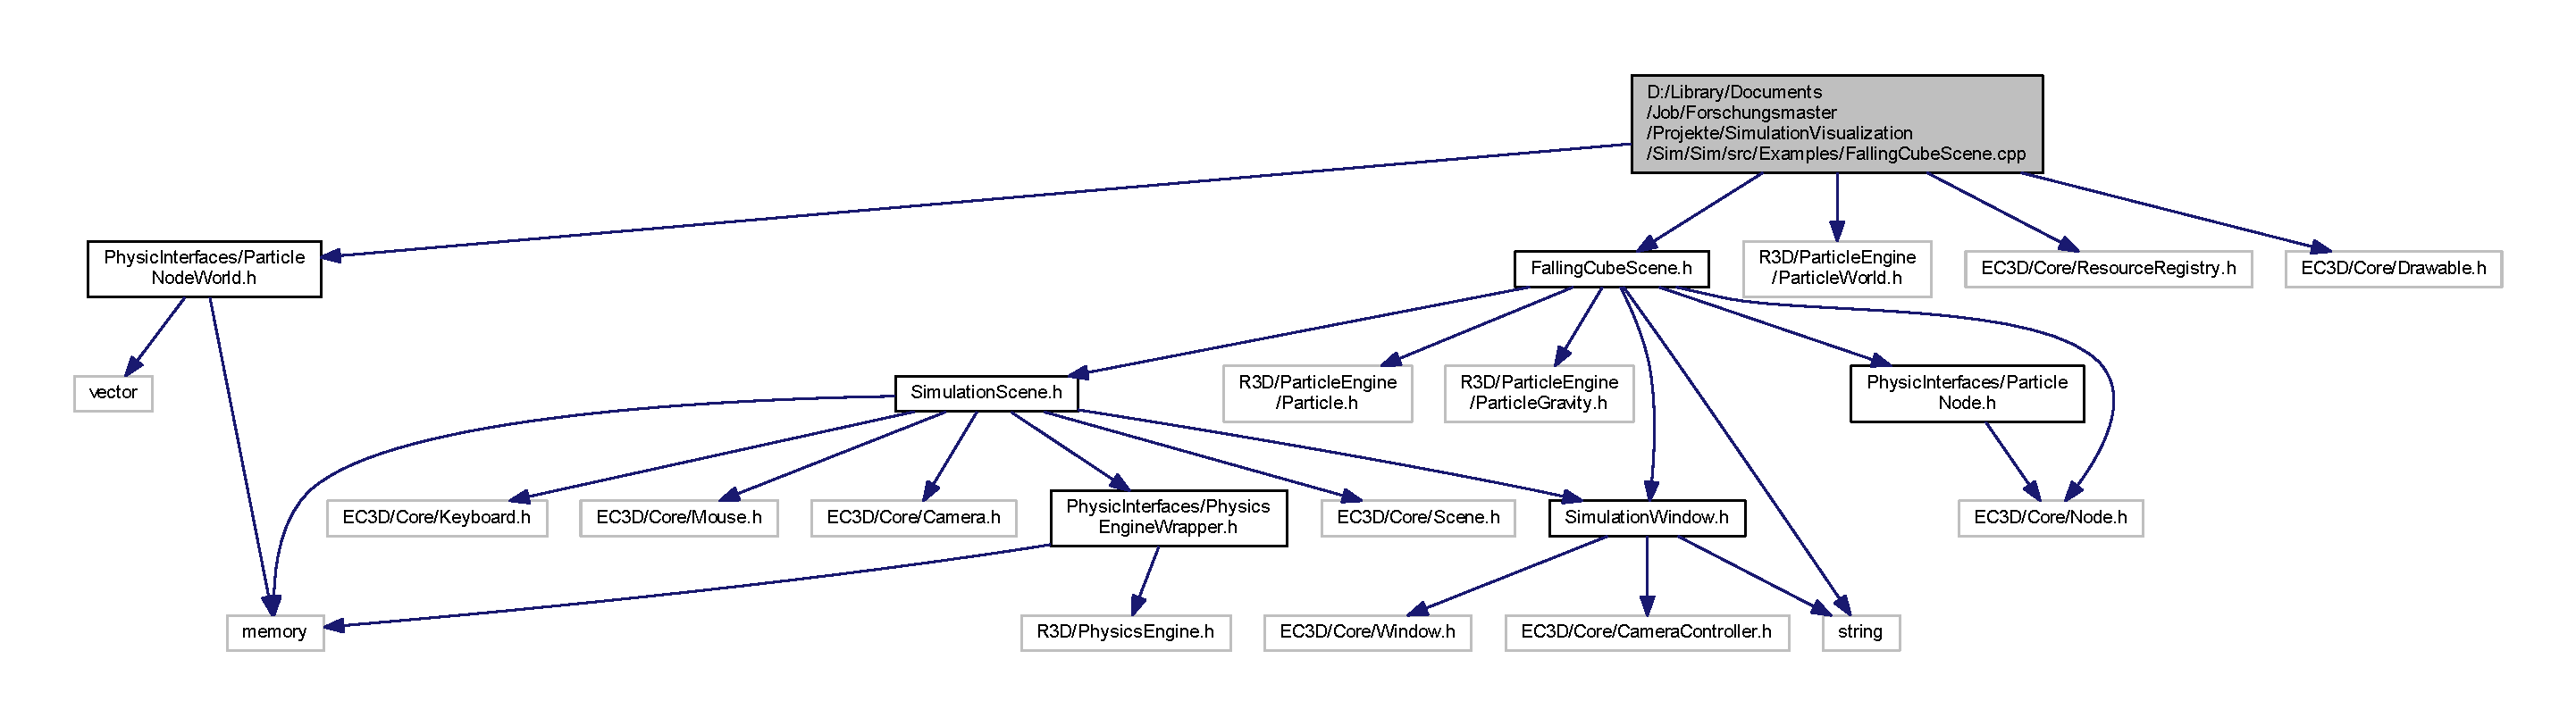
\includegraphics[width=350pt]{_falling_cube_scene_8cpp__incl}
\end{center}
\end{figure}
